\begin{figure}[htbp]
\centering
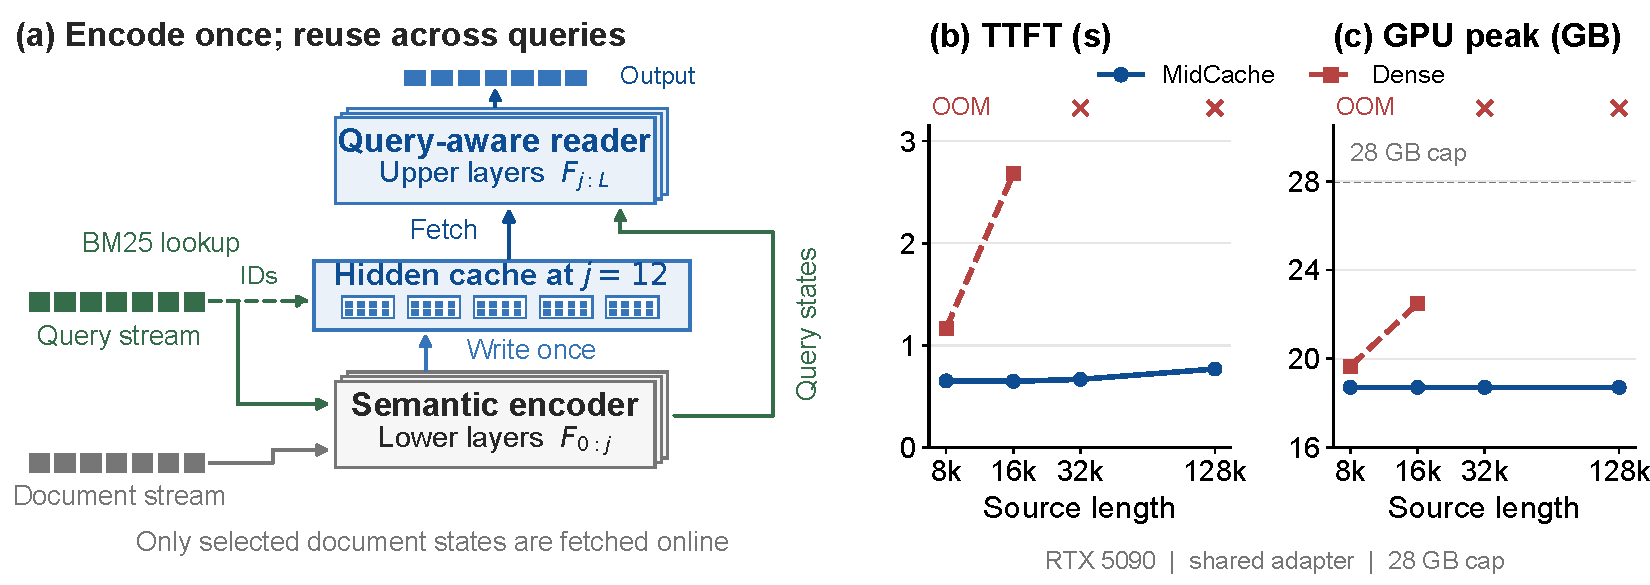
\includegraphics[width=\linewidth]{figures/teaser.pdf}
\caption{\textbf{A hidden cache between two parts of the LLM.} (a) The lower layers serve as a semantic encoder: their document states are cached once and reused by the upper reader. BM25 selects chunk IDs; only selected states are fetched. The query is also encoded before upper-layer continuation. (b--c) RTX 5090 measurements from Table~\ref{tab:infra}. TTFT includes retrieval, fetch, and query Write, but excludes document Write. GPU peaks include weights. Crosses mark actual Dense OOMs under the 28 GB allocator cap, without numerical values or extrapolation.}
\label{fig:teaser}
\end{figure}
